\begin{frame}[t]
 \frametitle{Fundamental Symmetries in Physics}
 \begin{block}<+->{Continuous local or gauge symmetries}
  \begin{itemize}
   \item Invariance under \alert{local transformations of the wave function}
   \item Lie groups of local transformations
   \begin{itemize}
    \item \alert{Unitary group $U(1)$}: complex numbers, absolute value 1
    \item \alert{Special unitary group $SU(n)$}: $n \times n$ unitary matrices, det 1
   \end{itemize}
  \end{itemize}
 \end{block}
 \begin{block}{Gauge fields for $U(1)$ under local phase change}
  \begin{itemize}
   \item Unobservable \alert{change of gauge fields} required
   \begin{center}
    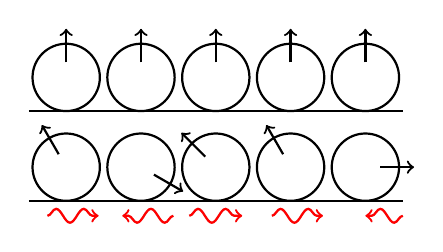
\begin{tikzpicture}[thick,scale=0.95]
     % Definitions
     \def\r{0.45}
     \def\off{0.2}
     \def\len{0.45}
     % Line and circles
     \def\y{0}
     \def\mycos{0}
     \def\mysin{1}
     \draw (0,\y) -- (5,\y);
     \foreach \x in {0.5,1.5,2.5,3.5,4.5} {
      \draw (\x,\y+\r) circle (\r);
      \draw[->] (\x+\off*\mycos,\y+\r+\off*\mysin) -- (\x+\off*\mycos+\len*\mycos,\y+\r+\off*\mysin+\len*\mysin);
     };
     % Line and circles
     \def\y{-1.2}
     \draw (0,\y) -- (5,\y);
     \foreach \x/\mycos/\mysin in {0.5/-0.5/0.866,1.5/0.866/-0.5,2.5/-0.707/0.707,3.5/-0.5/0.866,4.5/1/0} {
      \draw (\x,\y+\r) circle (\r);
      \draw[->] (\x+\off*\mycos,\y+\r+\off*\mysin) -- (\x+\off*\mycos+\len*\mycos,\y+\r+\off*\mysin+\len*\mysin);
      % Gauge fields
      \draw<1>[gray!30,->,decorate,decoration=snake] (\x+\mycos/2,\y-\off) -- (\x+\mysin/2,\y-\off);
      \draw<2>[red,->,decorate,decoration=snake] (\x+\mycos/2,\y-\off) -- (\x+\mysin/2,\y-\off);
     };
    \end{tikzpicture}
   \end{center}
  \end{itemize}
 \end{block}
\end{frame}
